% 2008 年安徽卷理科第 10 题：两个正态分布 N(μ1,σ1²)、N(μ2,σ2²) 的密度函数图象。
% 来源 PDF：gaokaomath-src/普通高考/2008/2008安徽理.pdf
% SHA-256：3493c8cb26596a78dafa0c1169fbdbfa4e69d8e593193f7c47128763b095c564
% 原页：2008安徽理.pdf 第 1 页（A3 三栏）第 2 栏，书页码 421。
% 重绘依据：按原页峰位与峰高重绘：左侧曲线峰约在 x=-0.5、高约 1.4（σ 较小），
%   右侧曲线峰约在 x=0.4、高约 0.85（σ 较大），坐标轴刻度 -1、-0.5、0、0.5、1 与 0.2～1.4。
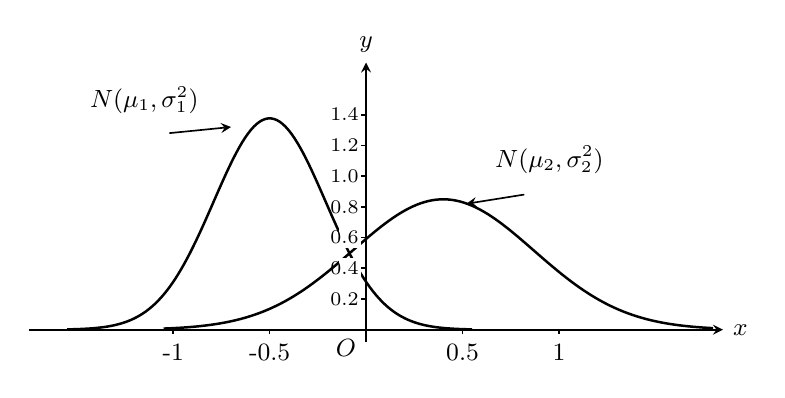
\begin{tikzpicture}[x=2.45cm, y=1.95cm, semithick, font=\small]
  \draw[->,>=stealth] (-1.75,0) -- (1.85,0) node[right] {$x$};
  \draw[->,>=stealth] (0,-0.08) -- (0,1.74) node[above] {$y$};
  \node[below left] at (0,0) {$O$};

  \foreach \x/\lab in {-1/-1, -0.5/-0.5, 0.5/0.5, 1/1} {
    \draw (\x,0) -- (\x,-0.03);
    \node[below] at (\x,-0.03) {\lab};
  }

  % 左：N(μ1,σ1²)，μ1≈-0.5，σ1≈0.29
  \draw[line width=0.9pt, domain=-1.55:0.55, samples=140]
    plot (\x, {1.376*exp(-((\x+0.5)*(\x+0.5))/(2*0.29*0.29))});
  % 右：N(μ2,σ2²)，μ2≈0.4，σ2≈0.47
  \draw[line width=0.9pt, domain=-1.05:1.80, samples=140]
    plot (\x, {0.849*exp(-((\x-0.4)*(\x-0.4))/(2*0.47*0.47))});

  \node[above] at (-1.15,1.34) {$N(\mu_1,\sigma_1^2)$};
  \draw[->,>=stealth] (-1.02,1.28) -- (-0.70,1.32);
  \node[above] at (0.95,0.95) {$N(\mu_2,\sigma_2^2)$};
  \draw[->,>=stealth] (0.82,0.88) -- (0.52,0.82);

  % 纵轴刻度与数字置于曲线之后，并以白色底遮断曲线，避免数字被曲线穿压
  \foreach \y in {0.2,0.4,0.6,0.8,1.0,1.2,1.4} {
    \draw (0,\y) -- (-0.03,\y);
    \fill[white] (-0.138,\y-0.068) rectangle (-0.028,\y+0.068);
    \node[left, inner sep=0.3pt, font=\scriptsize] at (-0.03,\y) {\y};
  }
\end{tikzpicture}
